% % Full page illustration
% \begin{figure}[!hbtp]
%     \centering
%     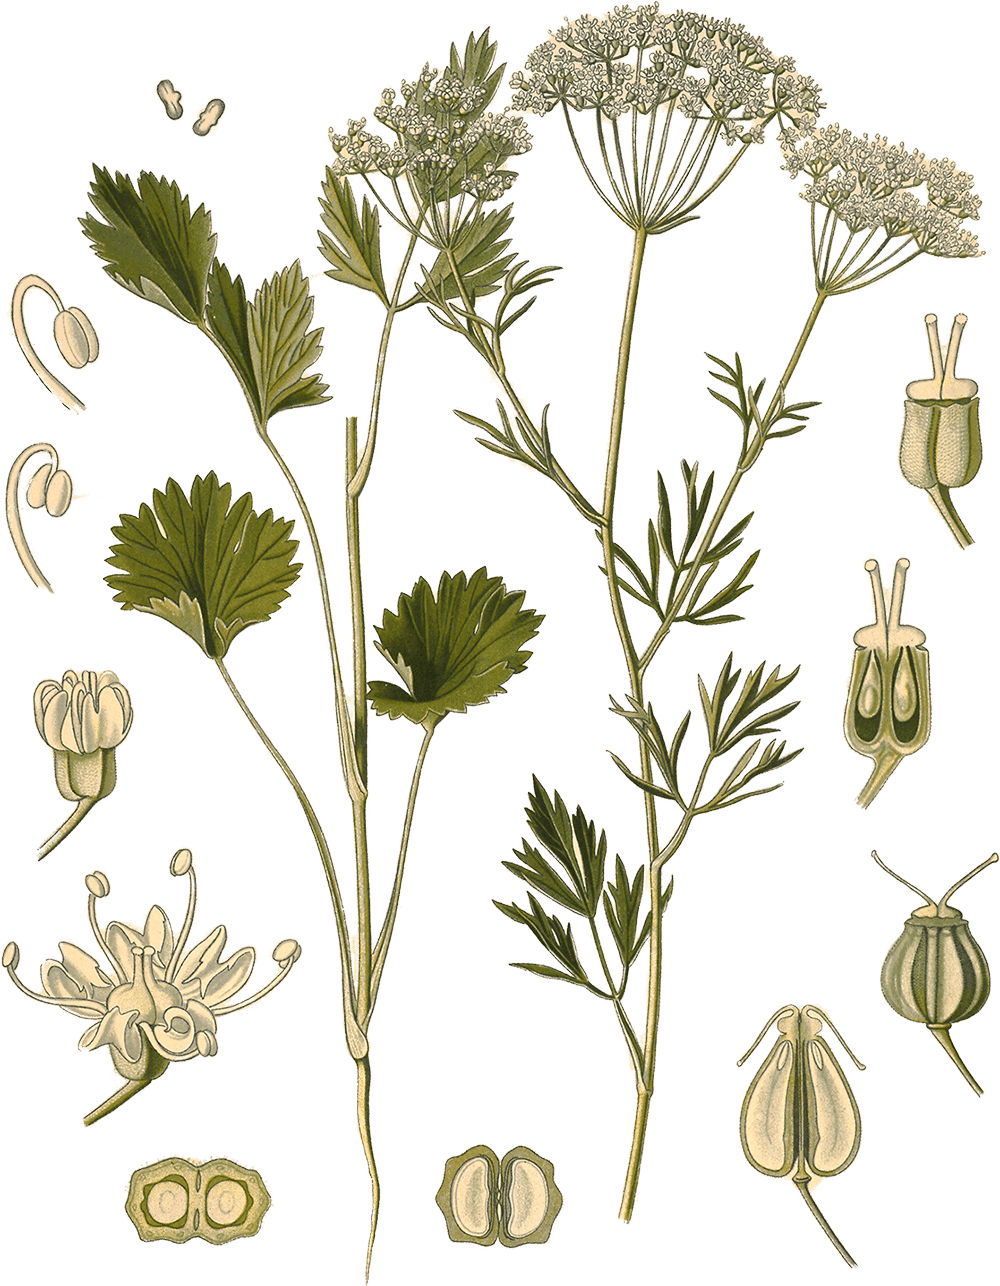
\includegraphics[width=\textwidth]{imgs/kohler/anise_kohler_min.png}
%     \caption{\taxonn{Pimenta dioica}{(L.) Merr.} (syn. \taxonn{P. officinalis}{ Lindl.}), the allspice tree in Köhler's Medicinal Plants \pvolcite[]{2}[174]{kohler_kohlers_1887}.}
%     \label{fig:kohler_anise}
% \end{figure}



\section{Anise}
\label{sec:anise}

\begin{spice}\label{spice:anise}
\textsc{Anise} \hfill \href{https://powo.science.kew.org/taxon/846658-1}{POWO} \\
\textbf{English:} \textit{anise}; \textit{aniseed}. 
\textbf{Arabic:} {\arabicfont{أنيسون}} \textit{anīsūn}; {\arabicfont{{يانسون} \textit{yānsūn}}}. 
\textbf{Chinese:} {\tradchinesefont{茴芹}} \textit{huíqín} [anise-celery]. 
\textbf{Hungarian:} \textit{ánizs}.  \\
\noindent{\color{black}\rule[0.5ex]{\linewidth}{.5pt}}
\begin{tabular}{@{}p{0.25\linewidth}@{}p{0.75\linewidth}@{}}
Plant species: & \taxonn{Pimpinella anisum}{L.} \\
Family: & \textit{Apiaceae} \\
part used: & fruit; oil \\
Region of origin: & E. Mediterranean; W. Asia \\
Cultivated in: & Turkey; Egypt; Spain; Russia; Italy; etc. \\
Color: & light brown \\
\end{tabular}
\end{spice}

% \begin{figure}[!ht]
% 	\vspace{-4ex}
% 	\centering
% 	\subfloat[\centering]{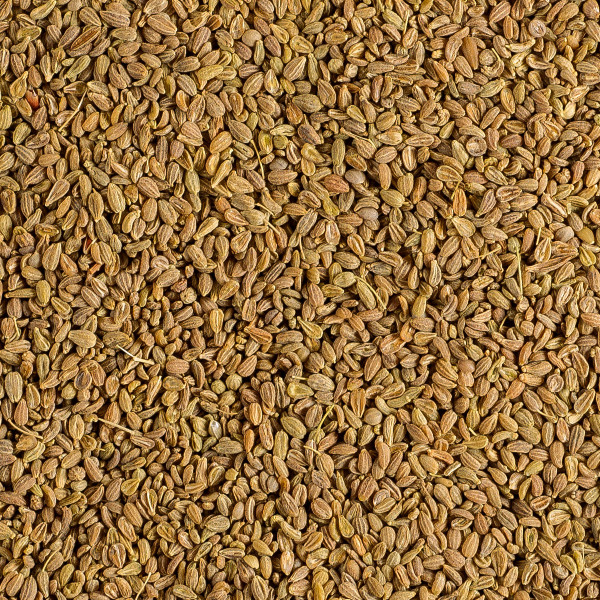
\includegraphics[width=0.3\linewidth]{imgs/spices/anise-1.jpg}}
% 	\hfill
% 	\subfloat[\centering]{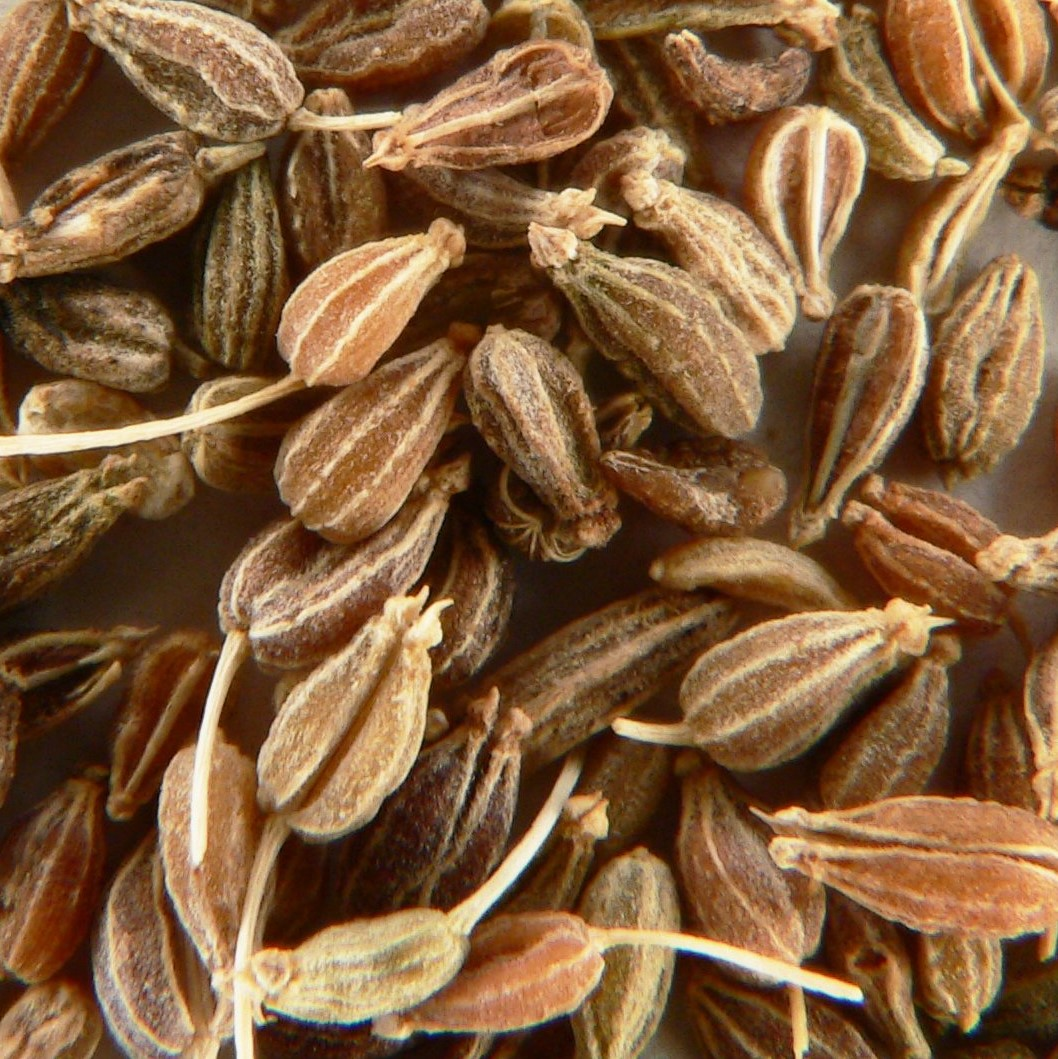
\includegraphics[width=0.3\linewidth]{imgs/spices/anise-11.jpg}}
% 	\hfill
% 	\subfloat[\centering]{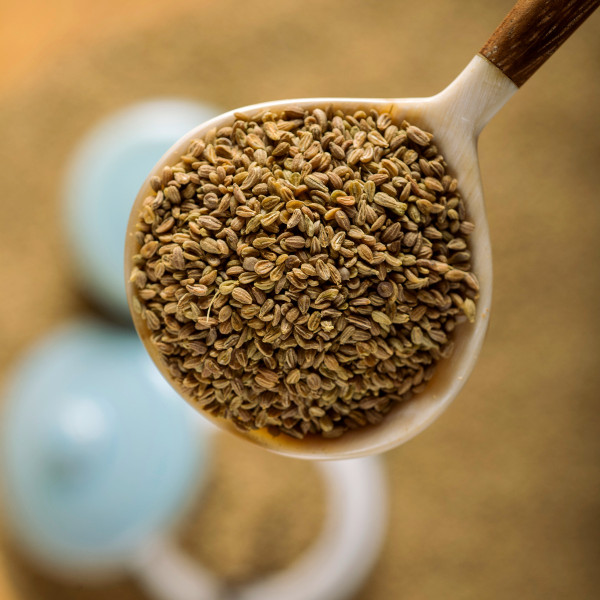
\includegraphics[width=0.3\linewidth]{imgs/spices/anise-3.jpg}}
% 	\caption{Anise \taxon{Pimpinella anisum}.}
% 	\label{fig:anise_imgs}
% \end{figure}

\begin{wrapfigure}{R}{0.33\textwidth}
	\vspace{-\baselineskip}
	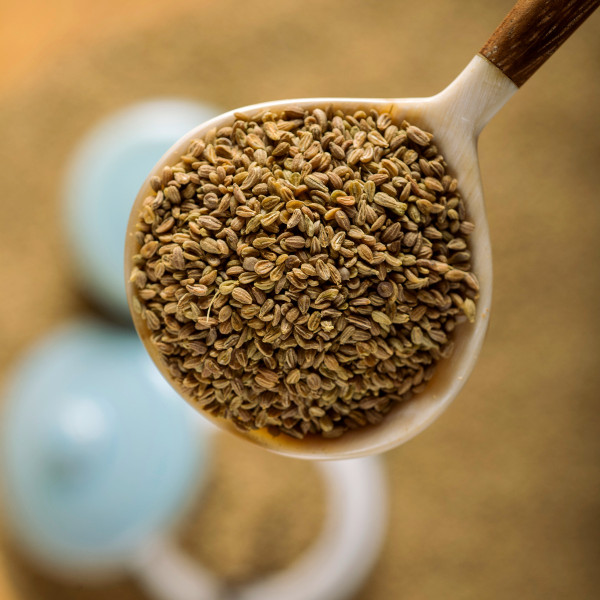
\includegraphics[width=0.33\textwidth]{imgs/spices/anise-s.jpg}
	\caption{Anise ``seeds'' (\taxon{Pimpinella anisum}).}
	\label{fig:anise}
\end{wrapfigure}

%DESCRIPTION

Anise (\taxon{Pimpinella anisum}) is a herbaceous plant, native to the Eastern Mediterranean and the Levant. It yields downy schizocarps,\footnote{Schizocarp refers to a dry compound fruit which splits into two or more one-seeded carpels (mericarps) without dehiscing} fruits which people call seeds. Hence the popular contracted form of the name, \textit{aniseed}. The seed-like fruits are grayish-green to light brown in color, and around 3--6 mm long \autocite[212]{van_wyk_culinary_2014}. Commercially available anise is usually sold whole, with a bit of stalk attached. Anise has visible \textit{vittae} (oil ducts) embedded in the fruit wall \pvolcite[]{2}[139]{peter_handbook_2012}, which is a feature similarly found on the fruits of related umbelliferous aromatic plants, such as fennel, cumin, caraway, carom/ajwain, and dill seeds.
Anise is sought after for its characteristic, liquorice-like sweet aroma and flavor, used in gastronomy, confectionery, and liqueur making -- especially around the Mediterranean. 
Anise and its essential oil is traditionally used as a flavoring for food, candy, and alcoholic drinks, however star anise oil from China has gradually replaced anise oil in the industry thanks to it being a much cheaper substitute \autocite[212]{van_wyk_culinary_2014}. % By 1999, world production in essential oil obtained from anise was 8 tons, while that of star anise was 400 \autocite{ashurst_food_1999}.

%OPERATIVE
The taste, smell, and even the appearance of anise resembles other---related and unrelated---spices, such as fennel, dill, liquorice, and star anise. This leads to a certain degree of confusion around the names which these plants and their products are known today in various languages. We will introduce this problem in more detail in \cref{sec:case_star_anise} in \nameref{ch:language}.

\begin{note}
	It is important to make the distinction between anise (\taxon{Pimpinella anisum}) and star anise (\taxon{Illicium verum}) from the beginning. These are two unrelated spices with distant origins. The similarities in name are due to their similarity in flavor, thanks to the organic compound anethole. 
	\end{note}

\subsection{The Botany, Origin, and  Cultivation of Anise}

%PLANT
Anise is an annual herb from the family \textit{Apiaceae/Umbelliferae}. Growing less than a meter tall, it brings small white flowers in umbels, the shape of an umbrella which is typical for this family of parsley, celery, and carrot. This family also contains many other aromatic flowering plants, such as asa\-foetida, coriander, cumin, caraway, dill, and fennel.

%ORIGIN
Anise originates in the Eastern Mediterranean region, growing from South East Turkey through Syria to the coasts of Lebanon, Israel, Palestine, and Egypt, including Cyprus, and in some sources also Greece. It has been cultivated since 2000 \BC{} \autocite[718]{mabberley_mabberleys_2017}.
%CULT
Anise today is naturalized in most of Europe and Central Asia, and it is cultivated as a crop in various regions around the globe, including, Southern Europe, Southern Russia, Turkey, the Middle East and North Africa, Pakistan, India, China, Chile, Mexico and the United States \autocite[32]{farrell_spices_1985}. It requires good soil, lots of sun and warmth, and also arduous to transplant. During harvest at summer's end when the fruits begin to ripen, the plant parts above ground are cut and the ``seeds'' are dried \autocite[212]{van_wyk_culinary_2014}.

\subsection{The History of Anise}

Anise has a long history around the Mediterranean, and its popularity is still concentrated there. It was used both as medicine an a culinary spice, as I mentioned above. The ancient Greeks took it as a breath freshener, and the Romans used it in their cooking \autocite{farrell_spices_1985}.

Pliny wrote a section of remedies with anise in his \textit{Natural History}, where he explains that it was recommended by Pythagoras to take with wine against scorpion stings, but it is also a great ingredient---both green and dried---in sauces and breads. And of course, it sweetens the morning breath with a little honey and smyrnion\footnote{\taxon{Smyrnium olusatrum}, an edible pot herb commonly known as \textit{alexanders}} \autocite[20:72 \link{http://www.perseus.tufts.edu/hopper/text?doc=Perseus\%3Atext\%3A1999.02.0137\%3Abook\%3D20\%3Achapter\%3D72}]{pliny_the_elder_natural_1855}.

Medieval European herbals tell of carminative effect: ``The seed wasteth and consumeth winde, and is good against belchings and upbraidings of the stomach, alaieth gripings of the belly, provoketh urine gently, maketh abundance of milke, and stirreth up bodily lust: it staieth the laske (diarrhea), and also the white flux (leukorrhea) in women.'' \autocite[880 \link{https://www.gbif.org/species/113561272}]{gerarde_herball_1597}. Based on modern research, anise oil and anethole is antibacterial, antifungal, antioxidant, carminative, and expectorant \pvolcite[]{2}[144]{peter_handbook_2012}.

The Brits and Arabs use it since the Middle Ages. According to \textcite{wilson_wedding_2005}, 
the tradition of the wedding cake grew out of the customary spiced cakes at the end of feasts during Roman times, which served as digestive. In modern Europe, its use is prevalent in confectionery (such as aniseed balls), but especially liqueurs. From the many Mediterranean alcoholic beverages flavored with anise, we can mention anisette and absinthe (made with \taxon{Artemisia absinthium}), from France, sambuca from italy, and ouzo and mastika from Greece. 
% ouzo effect
In the Eastern Mediterranean, it can be found in Turkish rakı, and the many araks of the Levant.

% USES
% culinary uses wyk
% Anise has a strong flavour and is used sparingly as a spice in soufflés, meat dishes (soups, stews, sausages), shellfish, vegetables (cabbage, carrots, turnips), mild cheeses, salad dressings, pickles, fruit dishes, desserts and juices. Chopped fresh leaves can be used in salads, pickled vegetables and fish soups. Star anise is nowadays often used as a substitute but connoisseurs say anise has a more delicate aroma. Anise is well known for its applications in confectionery (breads, biscuits, cakes and sweets) as well as alcoholic and non-alcoholic beverages. Examples of traditional culinary items and sweets are Australian humbugs, Austrian anisbögen, British aniseed balls, Dutch muisjes, German Pfeffernüsse and Springerle, Indian candy-coated saunf (used as mukhwas to freshen the breath after a meal), Italian pizzelle, New Mexican bizcochitos, New Zealand aniseed wheels, Norwegian knotts and Peruvian picarones. Well-known anise liqueurs or brandies/liquors (i.e.,respectively with or without sugar) include French anisette, pastis and Pernod, Greek ouzo, Middle Eastern arrack, Italian sambuca, Spanish anís and Turkish raki. These are drunk with a glass of water on the side or more often directly diluted with water, resulting in the familiar ouzo effect (the drink becomes cloudy and milky because the alcohol-soluble anethole is no longer fully soluble and forms an emulsion). 

%Flavour compounds
%The fruits contain 1−4% essential oil with (E)-anethole, also referred to as trans-anethole, as the dominant compound (up to 90% or more) and several minor ingredients such as cis-γ-himachalene, trans-pseudoisoeugenyl 2-methylbutyrate, methylchavicol and p-anisaldehyde.3 Anethole is a phytoestrogen that also occurs in fennel. 

%notes In Pakistani and Indian cuisine, no distinction is made between anise and fennel – both are called saunf. In Southeast Asia, the name for star anise is sometimes shortened to anis.

% Mebberley:
% P. anisum L. (anise, Greece to Egypt) – cult. since 2000 BC, food& drink-flavouring subs. for Artemisia absinthium (absinthe, anis, anisette, arak, ouzo, pastis, raki), distilled oil medic., familiar as aniseed balls;

\subsection{The Names of Anise}

\textit{Anise} is a typical \gls{wanderwort}: emerging from moderately obscure origins, it is now ubiquitous to the languages of Europe and its sphere of influence where it is culturally significant.

\subsubsection{English}

\begin{etymology}\label{ety:anise}
English \textit{anise}, ca. 1325
< French \textit{anis} `anise', 1236
< Latin \textit{anīsum} `anise', (dill is \textit{anēthum})
< Ancient Greek {ἄνισον} \textit{ánison} `anise; dill', and other Greek dialectal variants, e.g.: \textit{ánēthon}; included both plants, only later distinguished (probaby of substrate origin)
<\textss{?} Egyptian (Ancient) \textit{jnst} `a medicinal, edible plant (probably anise)'\footnote{\textcites[anise]{oed}[anise]{ahd}; \textcite[s.v. anis]{tlfi}; \textcite{lewis_latin_1879}; \textcite{liddell_greek-english_1940}; \textcites[99]{erman_worterbuch_1926}[240]{hemmerdinger_noms_1968}}
\end{etymology}

To English, it arrived in the \nth{14} century via French \textit{anis}, which descended from Latin \textit{anīsum}. The Latin word is a borrowing from Ancient Greek ἄνισον \textit{ánison}, which is attested in different forms in various Greek dialects of the time, sometimes with \textit{-nn-} and theta instead of sigma (e.g.,ἄνηθον \textit{anēthon}). We can often read that this word originally referred to dill, but it seems that the Greeks did not distinguish between the two, and the terms included both plants.\footcite[anise]{oed} Hence the scientific name of dill: \taxon{Anethum graveolens}. According to \textcite[103,107]{beekes_etymological_2010}, \textit{ánison} is anise, while \textit{anēthon} is dill, but he points out that they probably have the same etymon. The Romans borrowed both words, and the distinction was made explicit in \textit{anīsum} vs. \textit{anēthum}. The modern scientific names bear the Latin names: \taxon{Pimpinella anisum} (anise), where meaning of \textit{pimpinella} is uncertain, and \taxon{Anethum graveolens} (dill), where \textit{graveolens} means `strong scented' \autocite[184,303]{gledhill_names_2008}. The confusion of the Greek words had an effect on English much later as well, in Matthew 23:23 of the \gls{KJV}\footnote{Source: \url{https://www.biblegateway.com/passage/?search=Matthew+23\%3A23&version=KJV}} talks of anise, while newer, more accurate translations, such as the \gls{NRSV}\footnote{Source: \url{https://www.biblegateway.com/passage/?search=Matthew+23\%3A23&version=NRSVUE}} mention dill. In fact, one of the first attestation in English comes from Wycliffe's Bible in 1382, between mint and cumin: ``That tithen mente, anete [anese], and comyn.''\footcite[anise]{oed} Beyond Greek, the etymology of this word is uncertain, \textcite[103,107]{beekes_etymological_2010} suspects a pre-Greek, substrate origin demonstrated by the phonological variations. Although the \citetitle{erman_worterbuch_1926} in an early Egyptian glossary makes a connection with the Egyptian word rendered as \textit{jnst}\footnote{Transliterated as \textit{ꞽnś.t} in \textcite[99]{erman_worterbuch_1926}, conventional Egyptological pronunciation: /insɛt/} `an edible plant for medicinal use' in the literature of the Middle Kingdom, the assumption is marked with question marks in the original handwritten glossary \autocites[240]{hemmerdinger_noms_1968}[99]{erman_worterbuch_1926}. The \gls{AHD} remarks that the Greek word is ``perhaps from or akin'' to Egyptian \textit{ꞽnśt}---using a different transliteration---which is a kind of plant used in the preparation of refreshing drinks, possibly anise.\footcite[anise \link{https://www.ahdictionary.com/word/search.html?q=anise}]{ahd} 

% An association between dill and the ancient city of Imsety has been made due to the similarity of their names in Old Egyptian. Redford 1:562; more about jnst in Wiktionary

The idea is not far-fetched, anise, dill and other herbs are native to the region and were ``almost surely grown'' for their medicinal properties \pvolcite[]{2}[3]{redford_oxford_2001}. We know that spices and herbs were used to flavour Ancient Egyptian cooking, Egyptologists have identified indigenous ingredients (dill, fenugreek, parsley, thyme, nigella, fennel, marjoram, mint), those imported and transplanted from neighboring Palestine (dill, cumin, coriander, caraway) and those obtained through distant trade (cinnamon and peppercorns from Asia) by the wealthy, later during the New Kingdom times \pvolcite[]{1}[394,540]{redford_oxford_2001}.

Anise is also known as \textit{aniseed}, which is a contraction from \textit{anise} and \textit{seed}, a usage form that emerged in the late \nth{14} century. 

\textit{Sweet cumin} is another conventional name for anise, which shows the primacy of the word \textit{cumin} in English, when it comes to similar aromatic plants and their seeds. Cf. \textit{wild cumin}, \textit{Armenian cumin}, \textit{mountain cumin} (caraway); royal cumin\footnote{Parallel to Indo-Persian \textit{sh\={a}h-j\={i}r\={a} [king-cumin] `caraway'}} (bishop's weed), and the always ambiguous \textit{black cumin}

\begin{table}[!ht]
\centering
\begin{tabularx}{\textwidth}{@{}l>{\itshape \small}lL>{\small}l@{}}
\toprule
\textbf{\#} & \multicolumn{1}{l}{\textbf{Species}} & \multicolumn{1}{l}{\textbf{Name}} & \multicolumn{1}{l}{\textbf{Source}} \\
\midrule
\textbf{1}	& \textbf{Pimpinella anisum}	& \textbf{anise}	& \textbf{\textcite{van_wyk_culinary_2014}} \\
2	& Pimpinella anisum	& aniseed	& \textcite{van_wyk_culinary_2014} \\
3	& Pimpinella anisum	& sweet cumin	& \textcite{peter_handbook_2012} \\
\bottomrule
\end{tabularx}
\caption{Various names for anise in English.}
\label{table:names_anise_en}
\end{table}



\subsubsection{Arabic}

\begin{etymology}\label{ety:anisun}
Arabic {أنيسون} \textit{anīsūn} `anise', (later assimilated as \ar{يانسون} \textit{yānsūn}), a. 791
< Ancient Greek {ἄνισον} \textit{ánison} `anise; dill', and other Greek dialectal variants, e.g.: \textit{ánēthon}; included both plants, only later distinguished (probaby of substrate origin)
<\textss{?} Egyptian (Ancient) \textit{jnst} `a medicinal, edible plant (probably anise)', ca. 2030-1650 BC\footnote{\textcite{wehr_dictionary_1976}; \textcite{liddell_greek-english_1940}; \textcites[99]{erman_worterbuch_1926}[240]{hemmerdinger_noms_1968}}
\end{etymology}

In Arabic, similarly to English, the name of anise is a loanword from Greek. It is known by many spelling variations: \textit{anīsūn}, \textit{ānīsūn}, \textit{ansūn}, \textit{yānsūn}, and \textit{yansūn}. In general, the \textit{a-} forms were the initial loanword taken directly from Greek, then a \textit{y-} form emerged that assimilates better in Arabic phonology. In addition, synonyms for anise are \textit{kammūn ḥulw}, lit. `sweet cumin', and \textit{ḥubba ḥulwa} `sweet grain, sweet seed'.

Anise in Persian, is \fa{بادیان رومی} \textit\textit{bādyān rūmī}\footcite[Vol. 1, p. 197]{hayyim_new_1934}, literally `Roman anise', where \textit{bādyān} is an archaic word for either fennel or anise, the etymon of French \textit{badiane} that begot English \textit{badian} `star anise'. A possible connection between Persian \textit{bādyān} and Mandarin Chinese \zh{八角} \textit{bajiao} `star anise' have been proposed before, % by who
but in my opinion this is merely wishful thinking.

\begin{table}[!ht]
\centering
\begin{tabularx}{\textwidth}{@{}l>{\itshape \small}lr>{\itshape}lL>{\small}l@{}}
\toprule
\textbf{\#} & \multicolumn{1}{l}{\textbf{Species}} & \multicolumn{1}{l}{\textbf{Name}} & \multicolumn{1}{l}{\textbf{Tr.}} & \multicolumn{1}{l}{\textbf{Gloss}} & \multicolumn{1}{l}{\textbf{Source}} \\
\midrule
\textbf{1}	& \textbf{Pimpinella anisum}	& \textbf{أنيسون}	& \textbf{anīsūn}	& \textbf{phonetic}	& \textbf{\textcite{wehr_dictionary_1976}} \\
2	& Pimpinella anisum	& كمون حلو	& kammūn ḥulw	& sweet cumin	& \textcite{wehr_dictionary_1976} \\
3	& Pimpinella anisum	& يانسون	& yānisūn	& phonetic	& \textcite{wehr_dictionary_1976} \\
4	& Pimpinella anisum	& حبة حلوة	& ḥabba ḥulwa	& sweet grain, seed	& \textcite{wehr_dictionary_1976} \\
\bottomrule
\end{tabularx}
\caption{Various names for anise in Arabic.}
\label{table:names_anise_ar}
\end{table}



\subsubsection{Chinese}

\begin{etymology}\label{ety:huiqin}
Mandarin Chinese {茴芹} \textit{huíqín} `anise' [hui-celery], from \textit{hui} `anise/fennel' + \textit{qin} `celery' (茴 \textit{huí} could be interpreted as `Muslim spice', see 茴香 \textit{huíxiāng} `fennel'), 1841\footnote{\textcite{kleeman_oxford_2010; hu_food_2005}}
\end{etymology}

The gathering of names for anise is a bit difficult in Chinese for two reasons. Firstly, anise as a spice is relatively unknown in China except for Xinjiang, and therefore names are hard to find in sources. Since other spices with a similar flavour profile, such as the native star anise and the naturalized fennel are readily available, so anise was never imported into China. Consequently, we cannot find anise in reference works on Chinese food plants nor in Chinese \gls{materia medica} \autocite[see][]{hu_enumeration_1999, hu_food_2005}. It does however appear in the \gls{FOC}\footnote{Source: \url{http://www.efloras.org/florataxon.aspx?flora_id=2&taxon_id=200015767}} Secondly, identifications is problematic and confusing due to the mixing of terms \textit{anise}, \textit{aniseed}, \textit{star anise}, \textit{star aniseed}, etc. in English, and Chinese dictionaries, and in some databases as well. Dictionaries that do not give botanical names are of little help to clarify doubts, but some conclusions can be derived with care. Most dictionary entries in Chinese that translate \textit{anise} to \textit{aniseed} should in fact say \textit{star anise}, as they ar all words referring to the Asian spice, except for one: \zh{茴芹} \textit{huiqin}.

Anise in Chinese is 茴芹 \textit{huiqin} `anise-celery', which appears to be a relatively modern, scientific coinage, and the only \gls{phytonym} that appears in any publication (the \gls{FOC}). It is used in the strict sense of \taxon{Pimpinella anisum} and cannot be misunderstood for star anise (\taxon{Illicium verum}). It does not appear in historical corpora, and it is not included in the \nth{7} edition of the \textit{Xiandai Hanyu Cidian} [A Dictionary of Modern Chinese] \autocite[]{chinese_academy_of_social_sciences_xiandai_2016}, but it appears in the \gls{CEC}\footnote{Source: \url{https://dictionary.cambridge.org/dictionary/english-chinese-traditional/anise} and \url{https://dictionary.cambridge.org/dictionary/english-chinese-traditional/aniseed}.}, which gives us \textit{huiqin}, along with \zh{洋茴香} \textit{yanghuixiang} `Western anise'. \zh{茴香} \textit{huixiang} really refers to fennel, and the only reason it appears in \textcite{kleeman_oxford_2010} is the confusion between the materials, and their names. The nomenclature and the reasons behind its confusion will be explored in more detail in \cref{sec:case_star_anise}. A few other names are mentioned on the Chinese Wikipedia page of the plant, these all refer to the European origins of this spice, or referring to``Western Ocean'', the Indian Ocean used to denote foreign, western products that have arrived over sea.\footnote{Source: \url{https://zh.wikipedia.org/wiki/\%E8\%8C\%B4\%E8\%8A\%B9}}. 

A Latin-Chinese dictionary from a presbyterian missionary from 1841 lists \textit{huiqin} as \textit{thymus} `thyme',\footcite[715]{goncalves_lexicon_1841} which is rather confusing considering that 10 years earlier, the same author rendered it `oregano' in his Portuguese-Chinese dictionary.\footcite[585]{goncalves_diccionario_1831}. From this, we can speculate that more of the various spice herbs that the Portuguese and other Europeans brought to Macao were first denoted with \textit{huiqin}.

% oregano in 
% https://books.google.com.hk/books?id=BYE-AQAAIAAJ&pg=PA585&dq=%22%E8%8C%B4%E8%8A%B9%22&hl=en&sa=X&ved=2ahUKEwi1xs7slpb5AhWJet4KHe9NCicQ6AF6BAgEEAI#v=onepage&q=%22%E8%8C%B4%E8%8A%B9%22&f=false

% thyme in
% https://books.google.com.hk/books?id=rOBoAAAAcAAJ&pg=PA715&dq=%22%E8%8C%B4%E8%8A%B9%22&hl=en&sa=X&ved=2ahUKEwi1xs7slpb5AhWJet4KHe9NCicQ6AF6BAgJEAI#v=onepage&q=%22%E8%8C%B4%E8%8A%B9%22&f=false

\begin{table}[!ht]
\centering
\begin{tabularx}{\textwidth}{@{}l>{\itshape \small}ll>{\itshape}lL>{\small}l@{}}
\toprule
\textbf{\#} & \multicolumn{1}{l}{\textbf{Species}} & \multicolumn{1}{l}{\textbf{Name}} & \multicolumn{1}{l}{\textbf{Tr.}} & \multicolumn{1}{l}{\textbf{Gloss}} & \multicolumn{1}{l}{\textbf{Source}} \\
\midrule
\textbf{1}	& \textbf{Pimpinella anisum}	& \textbf{\tradchinesefont{茴芹}}	& \textbf{huíqín}	& \textbf{hui-celery}	& \textbf{\textcite{kleeman_oxford_2010}} \\
2	& Pimpinella anisum	& \tradchinesefont{茴香}	& huíxiāng	& hui-spice	& \textcite{kleeman_oxford_2010} \\
3	& Pimpinella anisum	& \tradchinesefont{西洋茴香}	& xīyánghuíxiāng	& western-ocean-hui-spice	& \textcite{wikipedia} \\
4	& Pimpinella anisum	& \tradchinesefont{洋茴香}	& yánghuíxiāng	& ocean-hui-spice	& \textcite{cec} \\
5	& Pimpinella anisum	& \tradchinesefont{歐洲大茴香}	& ōuzhōu dàhuíxiāng	& European-big-hui-spice	& \textcite{wikipedia} \\
\bottomrule
\end{tabularx}
\caption{Various names for anise in Chinese.}
\label{table:names_anise_zh}
\end{table}



\subsubsection{Summary}

\Cref*{table:names_anise} shows the names of anise that can be found in dictionaries.

\begin{table}[!ht]
\centering
\begin{tabularx}{\textwidth}{@{}ll>{\itshape}lLl>{\small}l@{}}
\toprule
\textbf{\#} & \textbf{Language} & \multicolumn{1}{l}{\textbf{Term}} & \textbf{Gloss} & \textbf{Loan} & \multicolumn{1}{l}{\textbf{Source}} \\
\midrule
1	& English	& anise	& 	& yes	& \textcite{oed} \\
2	& English	& aniseed	& 	& no	& \textcite{oed} \\
3	& English	& sweet cumin	& 	& no	& \textcite{oed} \\
\midrule
1	& Arabic	& anīsūn	& phonetic	& yes	& \textcite{wehr_dictionary_1976} \\
2	& Arabic	& kammūn ḥulw	& sweet cumin	& no	& \textcite{wehr_dictionary_1976} \\
3	& Arabic	& yānisūn	& phonetic	& yes	& \textcite{wehr_dictionary_1976} \\
4	& Arabic	& ḥabba ḥulwa	& sweet grain, seed	& no	& \textcite{wehr_dictionary_1976} \\
\midrule
1	& Chinese	& huíqín	& hui-celery	& no	& \textcite{kleeman_oxford_2010} \\
2	& Chinese	& huíxiāng	& hui-spice	& no	& \textcite{kleeman_oxford_2010} \\
\bottomrule
\end{tabularx}
\caption{Conventionalized names for anise in English, Arabic, and Chinese, found in dictionaries.}
\label{table:names_anise}
\end{table}













%==========================================

% EE:
% umbelliferous plant with aromatic seeds. XIV. — (O)F. anis :- L. ánīsum — Gr. ānīson.
% Hence aniseed XIV (anece seed).

% OE:
% anise (n.)
% Levantine plant cultivated for its seeds, which were important sources of chemical oils and flavoring, c. 1300, from Old French anis (13c.), from Latin anisum, from Greek anison. By the Ancients somewhat confused with dill. Related: Anisic.
% Entries linking to anise
% aniseed (n.)
% late 14c., a contraction of anise seed (n.).
% anisette (n.)
% "liqueur flavored with aniseed," 1821, from French Anisette de Bordeaux, from diminutive of anis (see anise).

% MW:
% Middle English anis, from Old French, from Latin anisum, anesum, from Greek anison, anēson
% First Known Use: 14th century (sense 1)

% AH:
% [Middle English anis, from Old French, from Latin anīsum, from Greek annēson, annīson, anīson; akin to anēthon, annēthon, dill, and perhaps from or akin to Egyptian jnś.t, a kind of plant used in preparing refreshing drinks (possibly anise).] 

% WK:
% From Middle English anys, borrowed from Old French anis, from Latin anīsum, from Ancient Greek ἄνισον (ánison), from Egyptian jnst. 
